\section{Pain}

Trigeminal Neuralgia is a chronic neuropathic facial pain syndrome. The quest for the understanding of the pathophysiology of this syndrome requires a review of the history and theories of pain. Pain is an unique and important sensory dimension that is central to the evolution and survival of animal species. In humans, the sensation of pain is typically described as an unpleasant quality. The experience of pain is complex, consisting of interaction between nociceptive, emotional and cognitive processes. The international association for the study of pain (IASP) defines pain as "An unpleasant sensory and emotional experience associated with actual or potential tissue damage, or described in terms of such damage"\footnote{http://www.iasp-pain.org/Taxonomy\#Pain}. 

Humanity have long sought to understand pain. In antiquity, thinkers in classical Greek traditions including Plato and Aristotle considered pain as primarily an emotion \cite{Moayedi2012a}. Hippocrates and Galen believed that pain arose from imbalances in vital fluids of the body, and considered the heart to be the organ responsible for the experience of pain \cite{Melzack1999}. These broad historical interpretations contrast more modern physiological approaches to the study of pain \cite{Melzack1999,Moayedi2012a}.

The earliest theory that attributes pain to a dedicated physical pathway is commonly credited to Ren\'{e} Descartes (\ref{fig:descarte}). However, for Descartes, pain as an experience  could not be divorced from the idea of the soul, as he had stated in his letter to the French polymath Marin Mersenne: "I do not explain the feeling of pain without reference to the soul. For in my view exists only in the understanding. What I do explain is all the external movements which accompany this feeling in us." \cite[p. 148]{BookCottingham1991v3}. In his \textit{Treatise of Man}, published in 1664, he stated: "Thus, for example, if fire A is close to foot B, the tiny parts of this fire...have the power also to move the area of skin which they touch. In this way they pull the tiny fibre which you see attach to it, and simultaneously open the entrance to the pore, located opposite the point where this fibre terminates -- just as when you pull one of a string, you cause a bell hanging at the other end to ring at the same time. When the entrance to the pore or small tube is opened in this way, the animal spirits from cavity enter and are carried through it...the fibres cause a movement in the brain which gives occasion for the soul...to have the sensation of pain" \cite[p.101-103]{BookCottingham1991v1}.

\begin{figure}[ht]

\includegraphics[width=0.3\textwidth]{descartes-reflex.JPG}
\centering
\caption{Illustration of Descartes' pain pathway from the Treatise of Man}
\label{fig:descarte}
\end{figure}

Descartes' description was the first instance where the experience of pain was considered from a mechanistic perspective. The pain percept was for the first time framed as a physical system that could be understood and potentially treated.

\subsection{Theories of Pain}
 
The concept of a pain specific pathway was first put forward by Charles Bell where he proposed that the brain is a heterogeneous structure, and that nerves are a mix of heterogeneous neurons that became bundled to facilitate anatomical distribution \cite{Bell1868}. Evidence soon followed with the discovery of specific touch receptors and the demonstration that resection of posterior spinal tracts in animals by Schiff and Woroschiloff isolated innocuous touch from pain and temperature conductance (anterolateral tract) \cite{Dallenbach1939}. Von Frey demonstrated distinct receptive fields that respond to pressure that triggered tactile, warm, cold and pain. Sherrington further developed the specificity theory by coining the term “nocicipient” and unified attributes of intensity theory and specificity theory \cite{Casey1982}.

The classic pattern theory on the other hand, as first proposed by John Paul Nafe in the 1929 paper “A quantitative theory of feelings”\cite{Nafe1929}, postulates that the pain is not mediated by a separate nervous system or specialized receptors, but rather by units of undifferentiated afferent nervous impulses that only vary in their numbers, spatial and temporal relationships, including impulse frequency, duration, and density of nerve unit activations. The pattern theory postulates that all bodily sensations are a result of the brain's interpretation of nervous impulses. The discovery of high threshold mechanoreceptors and unmyelinated nociceptors however discredited the pattern theory and gave further credence to the theory of specificity. 

The gate-control theory \cite{Melzack1965a} (\ref{fig:gate-theory}), which forms the basis of modern theory of pain, postulates that the cells of the substantia gelatinosa selectively inhibit signal transmission from primary afferent to the central transmission cells that relays touch or pain sensations. The transmission control depends on the large and small diameter primary afferents, where large fibers inhibit, while small fibers facilitate the transmission. The gate-control theory reconciles the two previously divergent specificity and pattern theories of pain.

 \begin{figure}[ht]
 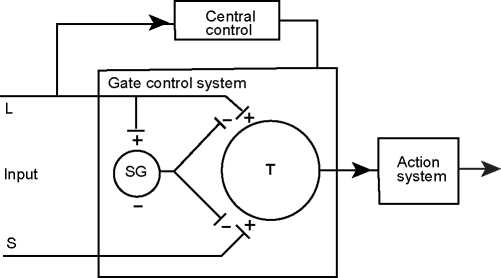
\includegraphics[width=0.8\textwidth]{gate-control.jpg}
 \centering
 \caption{Melzack's gate control theory diagram.}
 \label{fig:gate-theory} 
 \end{figure}
 
The key contribution of the gate-control theory was to emphasize the role of the dorsal horn in convergent pain processing, and therefore reconciles the evidences of pain-specific primary afferent and with pattern theory. The current theory of pain is defined such that the spatial and temporal profile of peripheral nerve activity encodes the necessary information for pain. That additional processing of information in the peripheral and central nervous system, both divergent and convergent, are in the form of patterns of cyclic nervous activities. This entire pattern of neural activities constitute the sensory component of the pain experience. Specifically, peripheral somatosensory and nociceptive pain afferents transmit to the spinal dorsal horn (laminae V), whereby wide-dynamic-range (WDR) neurons convergently process these primary afferents, and relay them to the thalamus, and subsequently the primary sensory cortex. A central concept, which was also introduced by Melzacks, is the pain neuromatrix, which dictates further cyclically convergent and divergent cortical patterns involving multiple cortical regions that in its entirety defines the entire pain perception \cite{Melzack1999}. (See section \ref{section:neuromatrix})


\subsection{Pain Physiology}

\subsubsection{Peripheral Receptors}

\textit{Nociceptors}, the receptors in the peripheral nervous system that detect tissue damage can respond to a range of electrical or chemical signals released by noxious stimuli on the tissue, such as physical trauma or heat/cold temperatures exceeding the pain threshold. These receptors broadly separate into two categories, differentiated by the type of axonal innervation they receive. Acute pain receptors are innervated by $A\delta$ fibres, which permits fast signal conductance (5 to 30 m/s) and trigger a prickly or sharp pain sensation; examples include needle prick other acute trauma. Dull pain is triggered by receptors that are innervated by slow conducting C fibres ($<1$ m/s). $A\delta$ and C fibres can be co-activated in the presence of noxious stimuli. 

\subsubsection{Nociception in the spinal cord}

The peripheral nociception signals are conducted from the axonal endings of the nociciption neurons, whose cell bodies are located in the spinal cord dorsal root gangions, to the dorsal horn of the spinal cord (\ref{fig:drg}). The $A\delta$ and C afferents project directly to lamina I of the dorsal horn. $A\delta$ afferents also directly project to lamina V. Lamina II, or the substantia gelatinosa, also receives inputs from C afferents, which indirectly synapse to lamina I neurons through interneurons. The dorsal horn also contains a dense layer of local interneurons in lamina III and IV, and receive input from innocuous somatosensory afferents at these layers. 

\begin{figure}[ht]
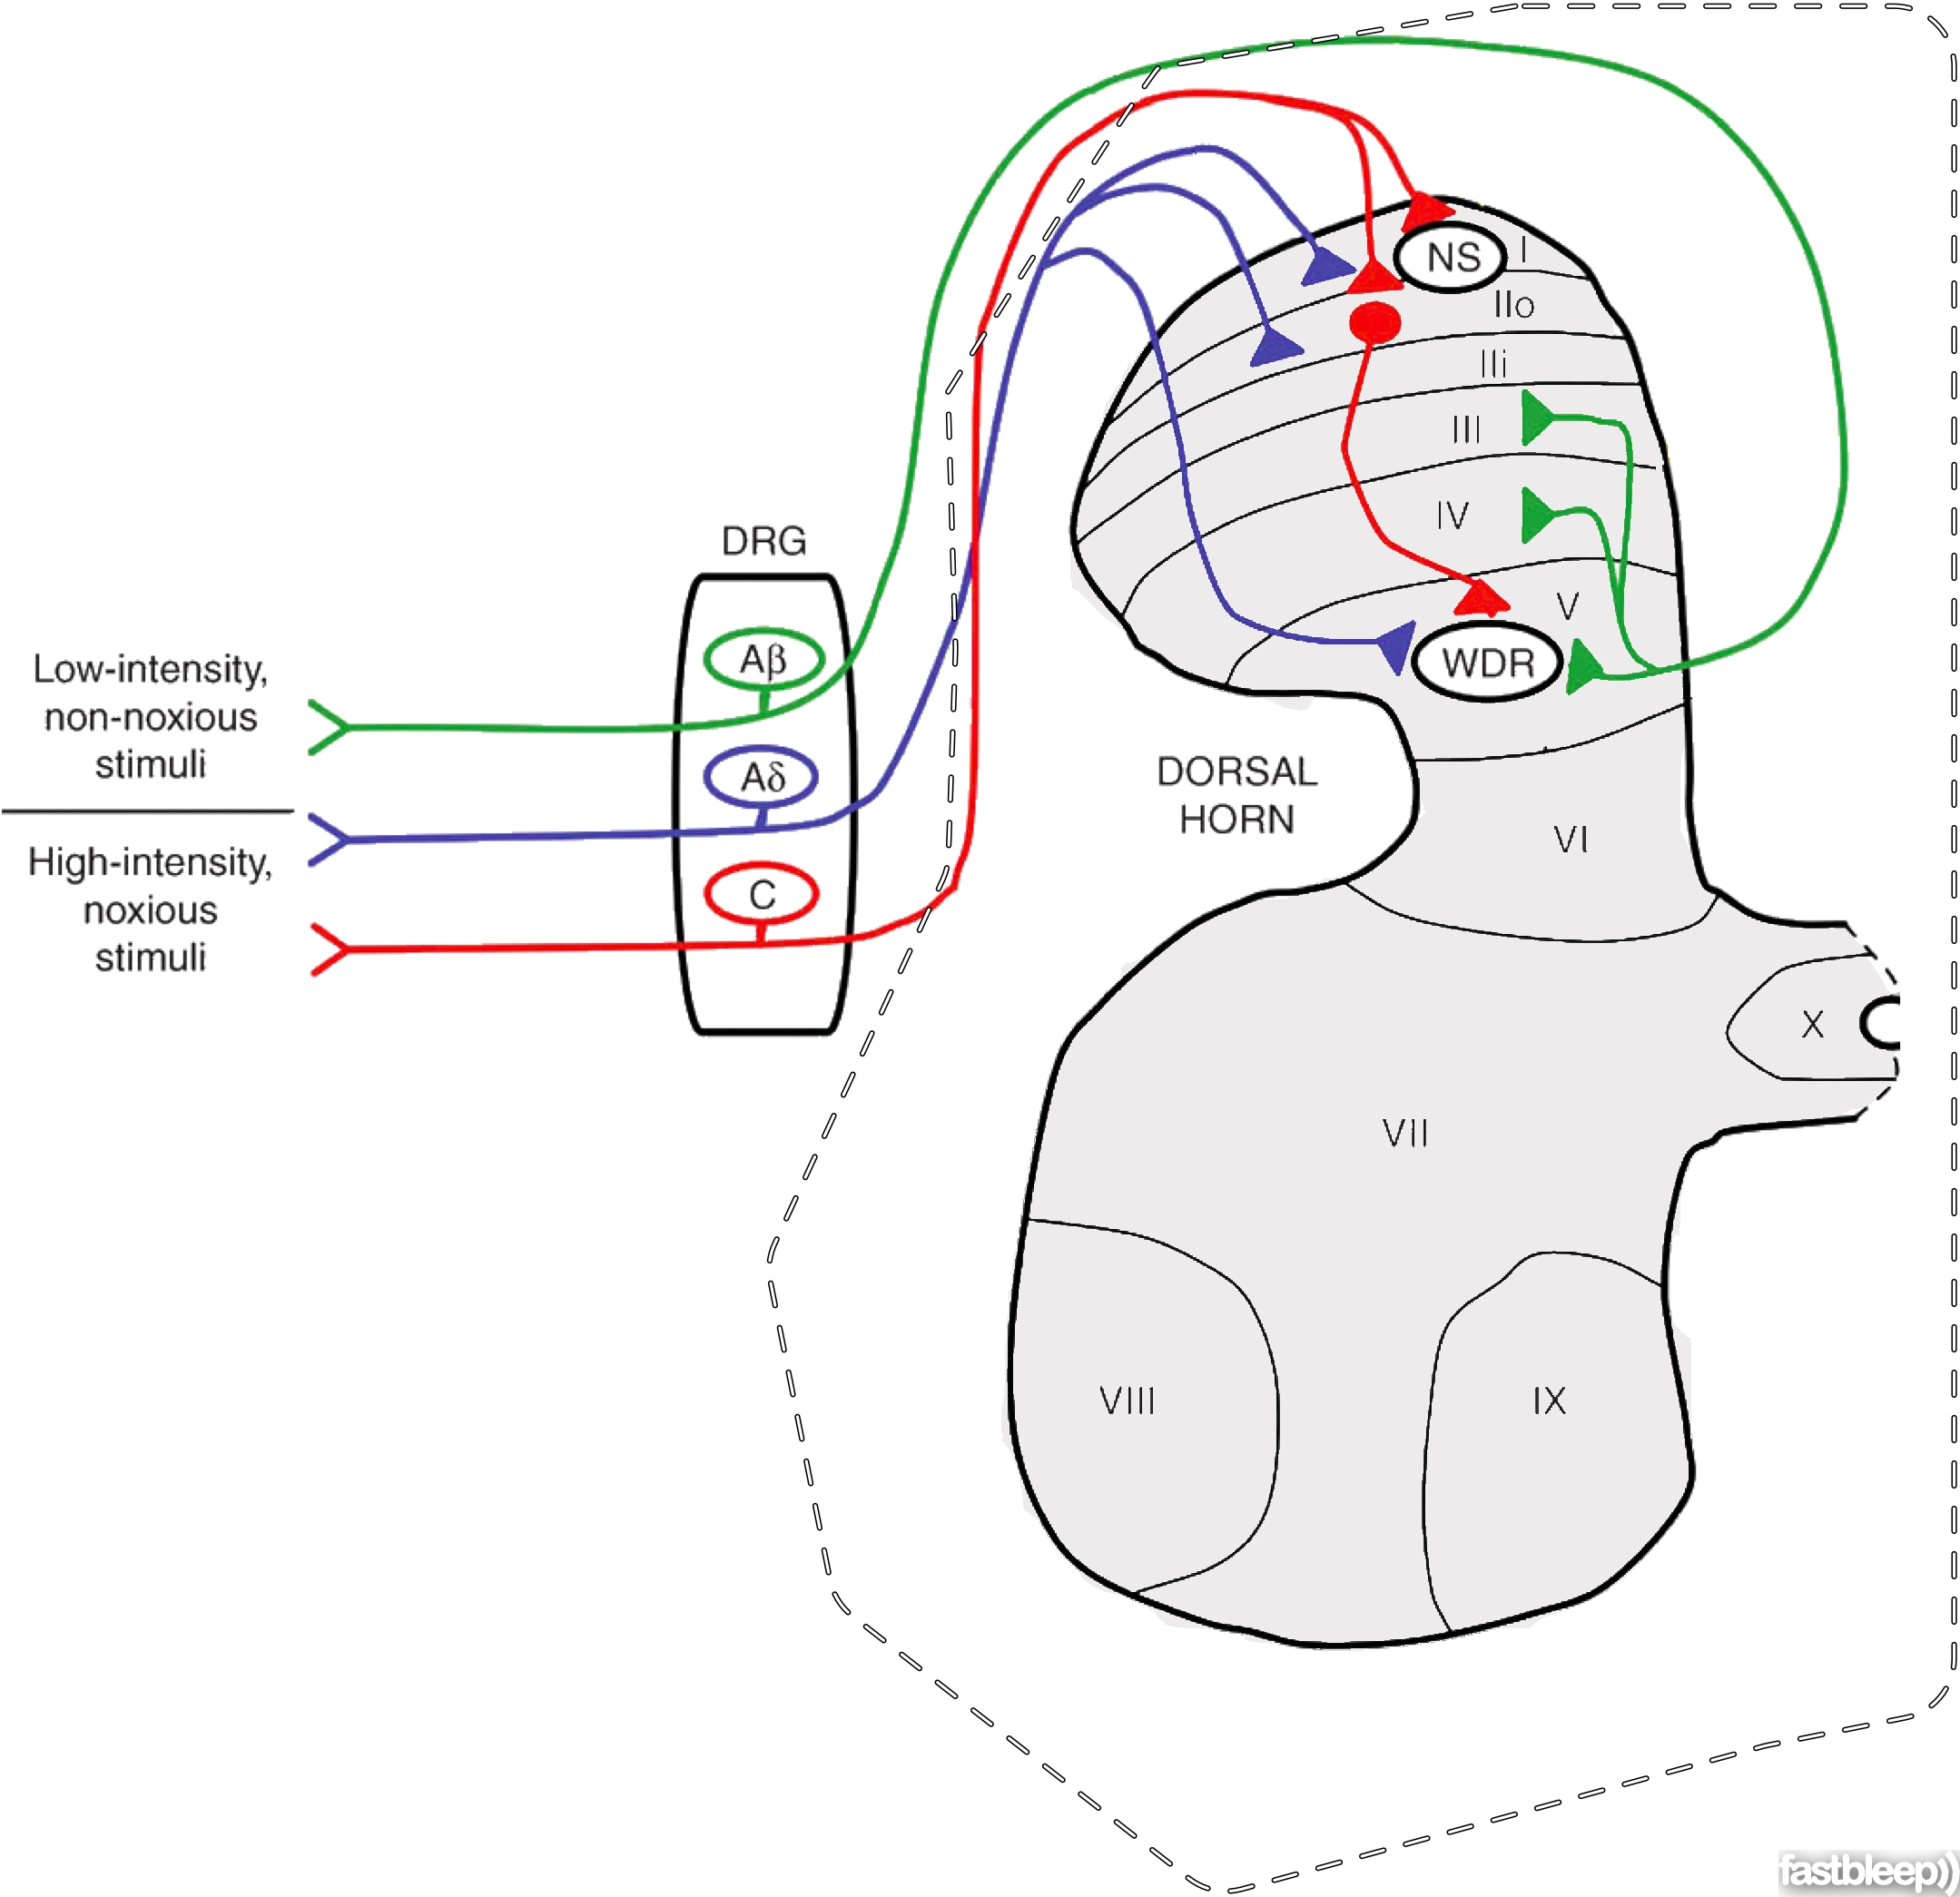
\includegraphics[width=0.8\textwidth]{pain-drg.jpg}
\centering
\caption{The axonal projections of the fast conduction ($ A\delta$) and slow conducting (C) pain stimuli in the dorsal horn.}
\label{fig:drg}
\end{figure}
 
The interneurons in the dorsal horn plays an important part in somatosensory integration as the sensory afferent pass from peripheral into the central nervous system. For example, the thermal grill illusion, discovered by Thunberg in 1896, involved the paradoxical feeling of heat or burning pain when adjacent skin regions are exposed to innocuous warm or cold stimuli \cite{Craig1994}. The mechanism is through the antagonistic interactions between innocuous cold A-fibers, cold heat pinch (CHP) C-fibers and warm C-fibers. Whereby the warm stimulus activates C-fibers that inhibit adjacent A-fiber activation, thereby unmasks the CHP C-fiber activations into the central nervous system.

Wide dynamic range (WDR) neurons are found primarily in the spinal dorsal horn in lamina V-VI. These neurons respond to both innocuous and painful stimuli, and are decidedly non-specific. They are found to sustain their impulse discharge during long durations of repetitive nociceptive stimulation, while nociceptive specific (NS) neurons showed a declined discharge rate within the same duration \cite{Coghill1993,Maixner1986}, thereby providing conclusive evidence that WDR neurons are sufficient for the percept of prolonged nociceptive pain. 

In each spinal afferent level, the dorsal horn neurons project noceciptive signals to the brain via five distinct paths (\ref{fig:pain-pathways}). Lamina I, V-VII axons crosses the mid-line to form the \textit{spinothalamic} tract that ascend in the contralateral anterolateral column of the spinal cord, and project to thalamic nuclei. Laminae VII and VIII neurons from the \textit{spinorecticular} tract ascend via the anterolateral quadrant of the spinal cord, without crossing the midline, to reach the reticular formation and thalamus. The \textit{spinomesencephalic} tract include axons from laminae I and V, and ascend in the anterolateral quadrant to the mesencephalic reticular formation, periaqueductual gray. The \textit{cervicothalamic} tract include only the white matters of the upper two cervical segments. It takes inputs from laminae III and IV, and projects to the thalamus via the medial lemniscus. The spinohypothalamic tract contains axons from laminae I, V, and VIII, and project to hypothalamic nuclei for autonomic functions. 

 \begin{figure}[ht]
 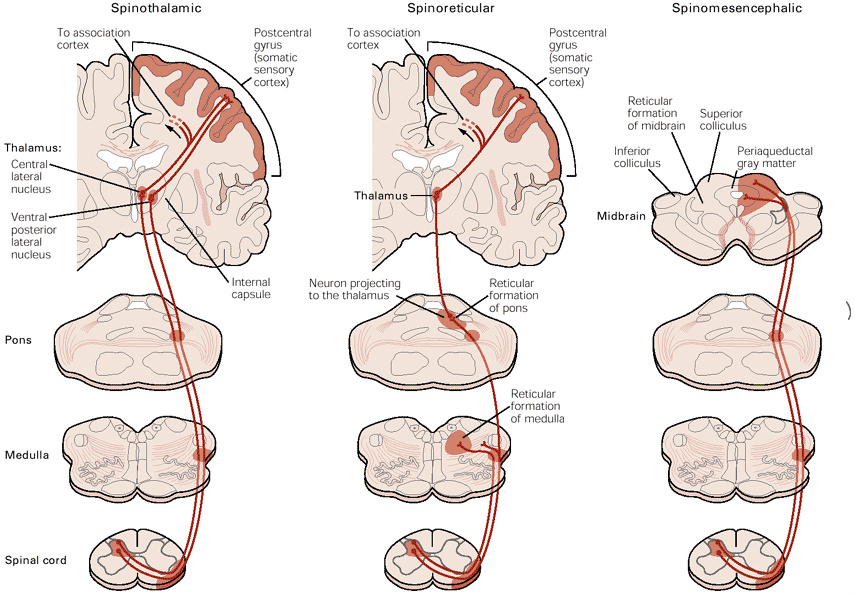
\includegraphics[width=\textwidth]{pain-pathways.jpg}
 \centering
 \caption{Afferent pain pathways} 
 \label{fig:pain-pathways}
 \end{figure}
 
 
\subsubsection{Thalamus}

Before reaching the neocortex, several important second order pain afferents arrive at the thalamus. The spinothalamic tracts subserving face and body sensory information terminate in the ventroposterior complex (VP, also known as ventrocaudal (Vc) nucleus), where ventroposterior-medial (VPM) nuclei and ventroposterior-lateral (VPL) nuclei are termination sites for face and body respectively. The VP complex sends third-order afferents to the primary sensory cortex (S1). Thus, the VP representation is somatotopically organized with the face region in the medial aspect, and lower limbs towards the lateral aspect. The representation is retained in the cortical projection, where the S1 somatotopy is shown to have the face region towards the lateral surface of the S1 cortical strip, and lower limb towards the superior-medial aspect. 

Another termination site is the mediodorsal (MD) nucleus of the thalamus, where pain afferents of the spinothalamic tract that originated from dorsal horn lamina I layer synapse. The MD nucleus projects third order afferents to the anterior cingulate cortex (ACC), which is shown to be prominent in the emotive/suffering cognitive aspect of pain.  

An important nucleus has thought to be unique in humans is the ventromedial-posterior nucleus (VMpo)\cite{Willis2002,Craig2014}. It receives afferents primarily from dorsal horn lamina I, and can be considered to be contiguous with the basal ventral medial nucleus (VMb), that forms a relay for homeostatic afferents \cite{Craig2003}. The VMPo projects to the dorsal posterior insular cortex, which is thought to involve body interoception of pain.

\subsubsection{Cortical projections of pain}\label{section:neuromatrix}

Pain percept, defined as the totality of the experience of pain, is thought to involve distributed regions of the brain, coined as the “pain neuromatrix”\cite{Melzack1999a}. The regions are not functionally independent, but rather thought to be dynamically inter-related. 

 Important cortical regions involved in pain include anterior cingulate cortex (ACC), insula, prefrontal cortex (PFC), thalamus, periaqueductal grey (PAG), secondary somatosensory cortex (SII) and motor cortex (M1). The role of these cortical regions in pain were discovered through neuroimaging fMRI studies \cite{Apkarian2013c,Wager2013,Davis2012a}, which demonstrated consistent BOLD co-activations during painful stimulation.
Regions such as ACC, PFC and insula are also shown to be active in social pain during social exclusion and emotional stress associated with PTSD revealed changes in ACC and insula grey matter (Section \ref{fig:pain-matrix}).

 \begin{figure}[ht]
 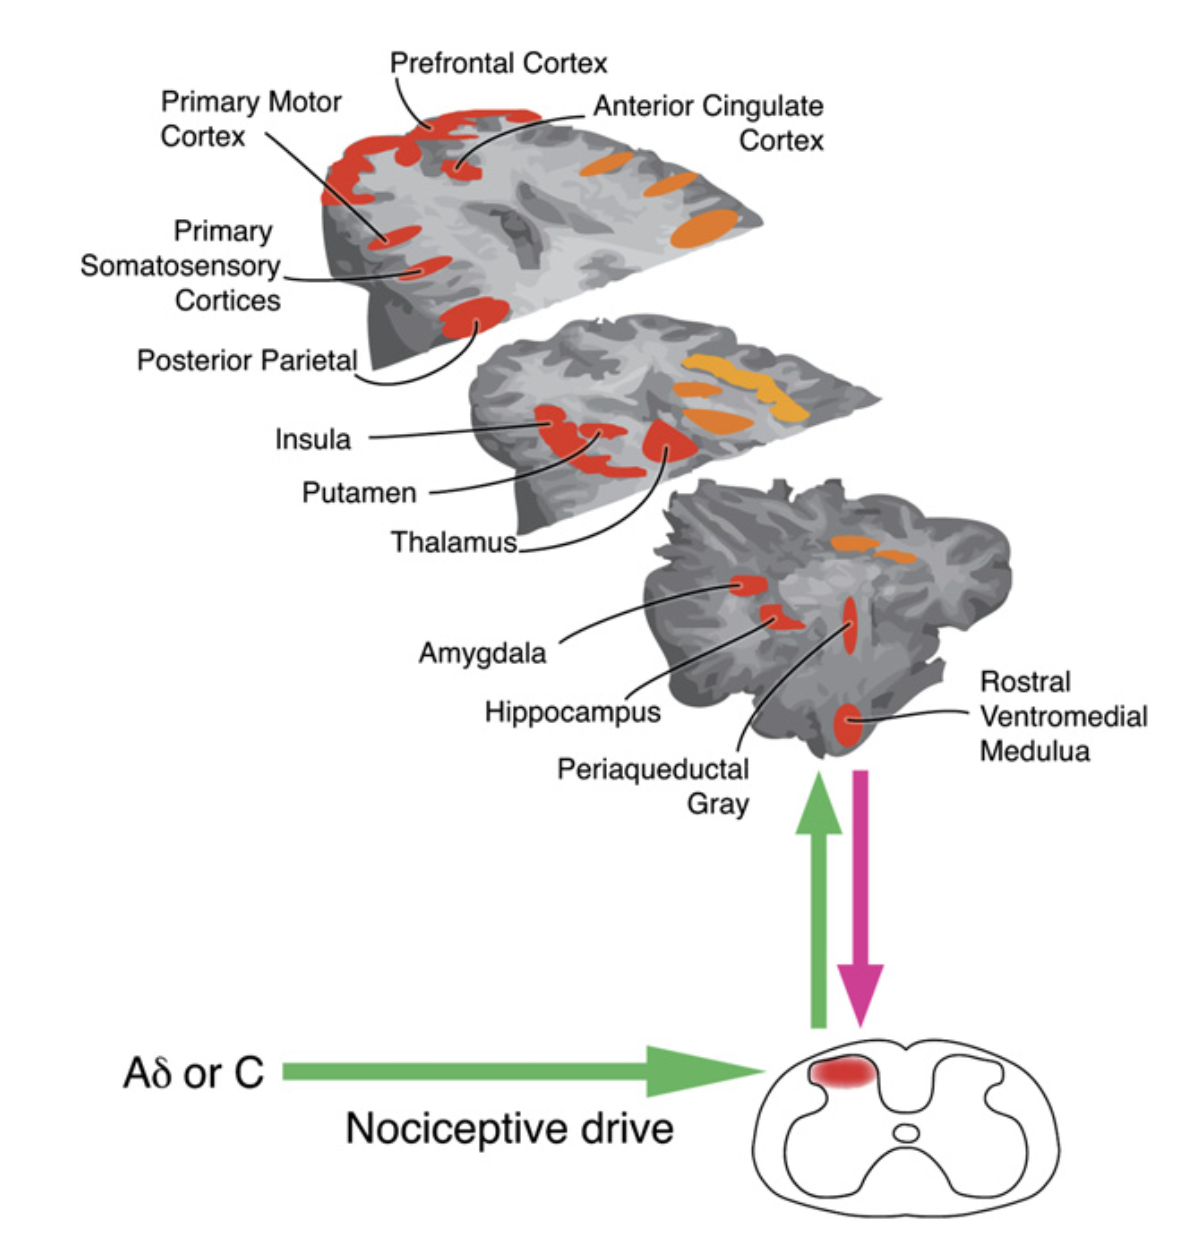
\includegraphics[width=0.8\textwidth]{pain-matrix.png}
 \centering
 \caption{Cortical and sub-cortical regions of the pain matrix.} 
 \label{fig:pain-matrix}
 \end{figure}
 
A recent study suggests that pain is correlated to the dynamically changing patterns of BOLD activities over time in the regions involved. Thus, the focus of the salient pain percept requires a switch away from the default mode network \cite{Kucyi2013}. The dynamic rhythms of activities that attune to and away from saliency, form a complex pain connectome \cite{Kucyi2015}. Conditions such as chronic pain therefore show a differentiated tuning of the default mode network and attention patterns of the brain due to their pathological activation of the pain matrix in the absence of detectable nociceptive stimuli \cite{Baliki2008,Legrain2009}.

\paragraph{Sensory-Discrimination}
Cortical regions associated with sensory-discriminative aspect of pain, such as the location and intensity of pain, include the primary sensory (S1) and secondary sensory (S2) cortices. The S1 cortex is responsible for the discrimination of fine-touch sensations. S1 receives inputs directly from VP thalamus. Nonetheless, S1 has not been consistently reported in acute pain studies, possibly due to the difficulty in detecting pain-related activations as there are relatively small number of nociceptive neurons within S1 \cite{bushnell1999pain}. S2, however, receives direct nociceptive input from VPI thalamus, and its BOLD activation is more consistently observed across pain fMRI studies. The posterior insula also receives direct nociceptive inputs from the VMPo thalamus \cite{Craig2003}, and shows strong functional and structural connectivity with S2 \cite{Wiech2014}. Therefore it is believe to plays an important role in pain sensory-discrimination. 

\paragraph{Affective-Motivational}
The cortical regions that are involved in affective-motivational pain procecssing, including unpleasantness and flight response, involve both regions that receive direct projection from the medial thalamus, as well as indirection regions. The anterior cingulate cortex (ACC) receives direct cortical projection from the medial dorsal nucleus, while the insula receives input from the VMpo thalamus. The amygdala is important for fight-flight reflex, and regions in the prefrontal cortices are believed to be related to the cognitive aspects of pain. These regions are demonstrated to correlate with the sensory-discriminative regions during the pain experience, but can be disassociated for example in pain empathy \cite{Singer2004}. 

\paragraph{Default mode network}
The default mode network (DMN) are regions of the brain, including the cingulate cortex, which show highly correlative BOLD activations in fMRI during wakeful rest \cite{Greicius2003,Raichle2015}. The core regions associated with the default network are ventral medial prefrontal cortex (vmPFC), posterior cingulate, inferior parietal, lateral temporal cortex, dorsal medial prefrontal cortex (dMPFC) and hippocampal formation. Regions such as vmPFC, dMPFC and the posterior cingulate overlap with the affective-motivational pain matrix, and are found to be disrupted in DMN in chronic pain \cite{Baliki2008}. DMN activation has been correlated with antinociception \cite{Kucyi2013} and it may undergo functional reorganization under chronic pain \cite{Baliki2014}. 

\paragraph{Insula}

The insula is an important neuroanatomical structure that has been implicated in both acute \cite{Lorenz2005,Starr2009} and chronic pain \cite{May2008,Jensen2016}. Anatomically it is subdivided into anterior and posterior components by the central insular sulcus. It can be further identified by its gyral features, consisting of 5 major gyri: anterior, middle and posterior short gyri in the anterior insula, and anterior long, posterior long gyri of the posterior insula. These gyri are not found consistently in the general population, but rather show individual variability \cite{Rosen2015}. Craig postulates that the insula is a key region for homeostasis and interoception \cite{Craig2003b}, and is necessary for pain discriminative sensations via VMpo projections in the middle insula in humans \cite{Craig2003a}. 

There is a recent debate pertaining the dorsal posterior insula as the "pain cortex" \cite{Segerdahl2015a}. Segerdahl et al. suggested that there is strong coupling between absolute cerebral blood flow and tonic pain intensity, and utilized arterial spin-labelling to quantify cortical activation in response to pain stimulation. The contralateral dorsal posterior insula emerged as the only cortical region with significant correlation. Tract tracing studies in monkeys has previously revealed pain-modality specific anatomy in the subregion of the dorsal posterior insula \cite{Craig2014}, and the study suggested that this is a strong supportive finding of a homologue region in humans. Critics of this finding raised issues with the low number of subjects, long sampling duration and the incompatibility of this interpretation with long standing bodies of neuroimaging literature \cite{Davis2015}. 

\subsection{Chronic Pain}

Chronic pain is pain that persists or recurrent past the healing phase following an injury \cite{Apkarian2009,Merskey2012}. It is more commonly defined as pain symptoms that persist longer than a fixed duration, most commonly 3 to 6 months, other factors to consider include psychosocial factors such as emotional and functional stress in addition to pain severity \cite{Treede2015}. The new ICD-11 revision of chronic pain classification include a new category for chronic primary pain. It is defined as "pain in one or more anatomical regions that persists or recurs for longer than 3 months, and is associated with significant emotional stress or significant functional disability" \cite{Treede2015}. It includes chronic pain conditions where the etiology is unknown. Conditions such as fibromyalgia, and irritable bowel syndrome fall under this category. Chronic pain conditions are considered to a type of maladaptive pain, whereby the pain response no longer serves its role in protecting the body from harm, but rather contributes negatively to the normal functions of life \cite{May2008}. 


\subsubsection{Neuropathic Pain}

Neuropathic pain is a type of chronic pain, defined as "pain caused by a lesion or disease of the somatosensory nervous system"\cite{Merskey2012}. The pain experience may be constant or paroxysmal, related to a stimulus (evoked) or spontaneous. Animal models of neuropathic pain suggest that peripheral and spinal circuitry responsible for the transmission of nociception are altered under pathological conditions. The nervous system is believed to be altered by maladaptive plasticity following a nervous system insult thereby resulting in sustained neuropathic pain.

The maladaptive mechanism responsible for neuropathic pain may manifest in any stage of the nociceptive transmission and processing circuitry. 
Noxious signal arises in the periphery, and undergoes signal transformation in the periphery and spinal ganglions, and is then subsequently processed as the pain percept in the neocortex. The pain percept is also modulated by emotional and cognitive factors, which triggers downstream modulation that ultimately affects the nociceptive signal transformation. 

Peripheral neuropathic pain often occurs after lesion to the peripheral nervous system, and can be caused by physical trauma and infections. Central neuropathic pain is caused primarily by lesions in the central nervous system, including spinal cord injury, lesions relatting to multiple sclerosis or tumours. 


\paragraph{Peripheral Sensitization}

Peripheral neuropathic pains can arise when there are disruptions in peripheral signal transmission. The disruption can be a result of injury to the first order peripheral afferent neurons, which result in increased sensitivity to stimuli and via ectopic action potentials. Changes in peripheral neurotropic factors as a result of an injury can cause increased membrane excitability or spurious sprouting of the synaptic terminals in the dorsal horn of the spinal cord. Additionally, maladaptive changes may occur in the secondary sensory neurons and interneurons in the dorsal-horn laminae that amplifies or reroutes the noxious signals \cite{Elmes2004}.

\paragraph{Central Sensitization}

Neuropathic pain can also arise from changes in the central neuroaxis. Trauma and other disruptions to the spinal pathways can affect noxious signal transmission. White matter pathways within the brain may also become damaged by conditions such as trauma, infections, and multiple sclerosis, such that the synchronicity of action potential conduction between cortical and subcortical structures are disrupted, and thereby give rise to neuropathic pain. It is believed that injury to white matter fibers can affect action potential conduction between cortical and subcortical structures. This may give rise or contribute to neuropathic pain \cite{Geha2008}.

 The utilization of magnetic resonance imaging (MRI), coupled with novel imaging modalities such as functional MRI (fMRI) and diffusion MRI (dMRI), have been instrumental in our understanding of pain, permitting both \textit{in vivo} measures of brain activity during pain (functional studies) \cite{Davis2006}, as well as assessment of changes to the brain microstructure \cite{Hodaie2009a,Chen2015c}.
 
 Neuropathic and acute nociceptive pain have a high degree of overlap in brain activations \cite{Moisset2007}, therefore differentiating between neuropathic and acute pain from neuroimaging continue to be an active area of research. Brain regions that are involved in the somatosensation of pain process are involved in both acute and chronic pain. These regions include the posterior insula, lateral thalamus and dorsal striatum. In chronic pain conditions however, there is increased activation in the anterior insula, ventral striatum, orbital frontal cortex and dorsal lateral prefrontal cortex \cite{Lorenz2005}. In chronic back pain, diffusion changes in fractional anisotropy was correlated with medial prefrontal cortex and nucleus accumbens connectivity in pain recovery, but not when the pain persistented \cite{Mansour2013}. Evidence also suggest that back pain chronification seem to increase activation in the emotional regions (amygada and medial prefrontal cortex) of the brain, and transition away from sensory region activations \cite{Hashmi2013}. A shift in forebrain activities is observed in neuropathic versus acute pain, abnormal activities in anterior cingulate cortex and prefrontal cortex is commonly observed in these studies \cite{Davis2006}. 
 
 Advances in modern machine learning methods led to their uses in attempting to improve neuropathic pain classification and diagnosis. Modern approaches combines cross-modal and additional analytical features, and can involve fMRI, diffusion imaging, as well as functional and/or structural connectivity. Machine learning in the form of multivariate pattern analysis to classify individuals with chronic back pain from normal controls, and achieve 92\% accuracy \cite{Callan2014}. Other studies in chronic pelvic pain using linear support vector machine was able to achieve 73\% accuracy \cite{Bagarinao2014}. Differentiating neuropathic and acute pain however is more difficult. Functional connectivity based classification on differentiating fibromyalgia, rheumatoid arthritis and controls was able to achieve a diagnositc accuracy of 69\%, and classification accuracy of 78\% \cite{Sundermann2014}.    
 
 